\documentclass[12pt]{article}
\usepackage[margin=1in]{geometry} 
\usepackage{amsmath}
\usepackage{tcolorbox}
\usepackage{amssymb}
\usepackage{amsthm}
\usepackage{lastpage}
\usepackage{fancyhdr}
\usepackage{accents}
\usepackage{mathtools}
\usepackage{tikz}
\usepackage{gensymb}
\usepackage{listings}
\usepackage{graphicx}
\usepackage{circuitikz}
\usepackage{pgfplots}
\pagestyle{fancy}
\setlength{\headheight}{40pt}

\lstset{
  basicstyle=\ttfamily,
  columns=fullflexible,
  frame=single,
  breaklines=true,
  postbreak=\mbox{\textcolor{red}{$\hookrightarrow$}\space},
}

\newenvironment{solution}
  {\renewcommand\qedsymbol{$\blacksquare$}
  \begin{proof}[Solution]}
  {\end{proof}}
\renewcommand\qedsymbol{$\blacksquare$}

\newcommand{\ubar}[1]{\underaccent{\bar}{#1}}

\usetikzlibrary{calc,patterns,angles,quotes}

\title{Quantitative Engineering Analysis \\ Bridge of Doom}

\author{Rohil Agarwal, Wesley Soo-Hoo \\ Olin College of Engineering \\ ENGX2001 Spring 2020}
\date{\today}

\begin{document}
\begin{titlepage}
\maketitle

\begin{center}
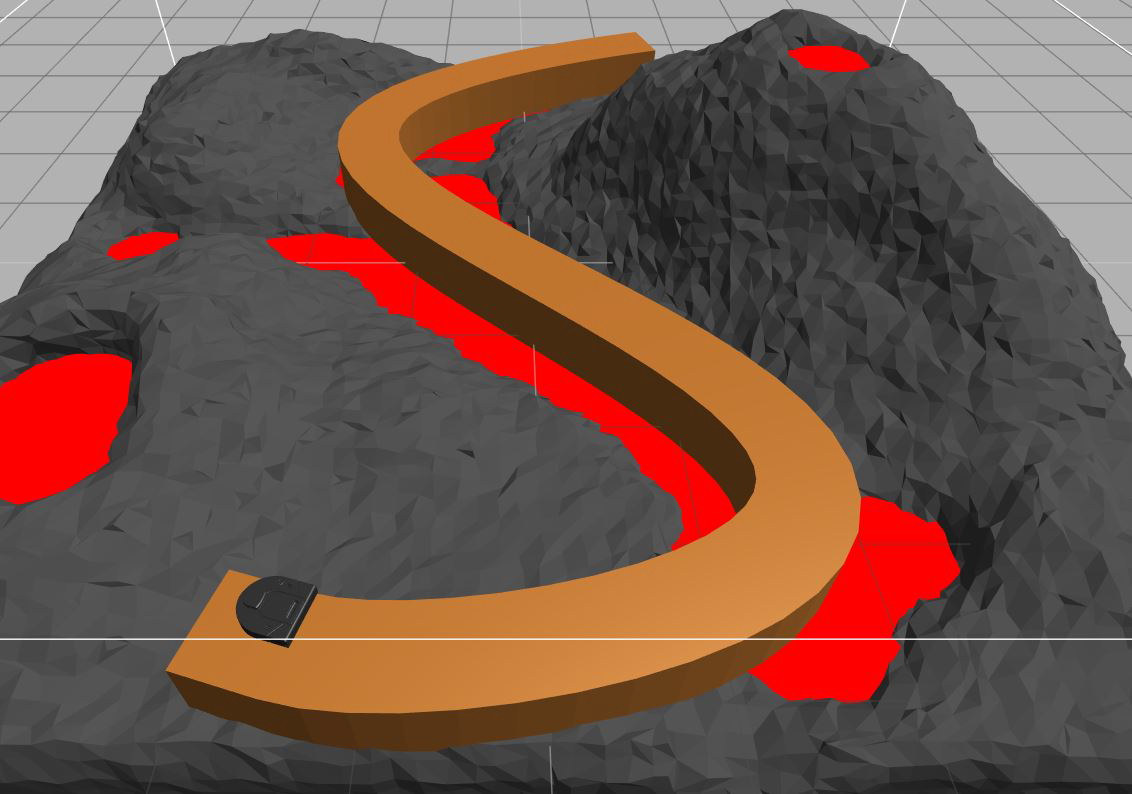
\includegraphics[width=.75\textwidth]{img/cover.png}
\end{center}
\end{titlepage}

\section{Introduction}
The Bridge of Doom is an arbitrarily shaped bridge suspended above a volcano. The challenge is to write a program to command a Neato, a robotic vacuum cleaner, to cross this bridge without falling off. 

The centerline of the Bridge of Doom can be described by a parametric curve. Using this definition, it is possible to determine the vectors that are tangent and normal to the curve at each point along the curve. These vectors can then be used to determine the ideal linear speeds, angular velocities, and wheel velocities that the robot should move with at given points in time in order to safely make it across the bridge.

\section{Methodology}
\subsection{Planning}
The bridge was represented with the parametric curve:

\begin{align*}
    \boldsymbol{r}(u) = 4 \times 0.396 \cos(2.65 (u + 1.4)) \boldsymbol{\hat{i}} - 4 \times (0.99 \sin(u+1.4)) \boldsymbol{\hat{j}}, (u \in [0, 3.2])
\end{align*}

A plot of the predicted path is seen in \textbf{Figure \ref{fig:both_paths}}.

The parametric equation was then used to find the velocity vectors of the path, which is then used to find the linear speeds and the angular velocities of the robot as a function of time.

\begin{align*}
    \boldsymbol{v}(u) &= \frac{dr}{du} \\
    \boldsymbol{\hat{T}} &= \frac{v}{|v|} \\
    \boldsymbol{V_T}(u) &= \boldsymbol{\hat{T}} \cdot \boldsymbol{v}(u) \\
    \boldsymbol{\omega}(u) &= \boldsymbol{\hat{T}} \times \frac{d\boldsymbol{\hat{T}}}{du}
\end{align*}

The linear speed and angular velocities are plotted in \textbf{Figure \ref{fig:planned_lin_ang_speeds}}.

Finally, the planned left and right wheel velocities were calculated using the equations for differential drive.

\begin{align*}
    \boldsymbol{V_L}(u) &= \boldsymbol{V_T}(u) - \frac{d\boldsymbol{\omega}(u)}{2} \\
    \boldsymbol{V_R}(u) &= \boldsymbol{V_T}(u) + \frac{d\boldsymbol{\omega}(u)}{2} \\
\end{align*}

where $d$ is defined as the distance between the left and right wheels, in meters. The $d$ constant of the Neato is 0.235.

The wheel speeds are plotted in \textbf{Figure \ref{fig:planned_wheelspeed2}}

One key takeaway of this model is that it shows the maximum speed (assuming $u$ is time) is almost $6 \frac{m}{s}$. The maximum wheel speed of a Neato is defined as $2 \frac{m}{s}$. Because of the initial planned speed is greater than the maximum speed of the Neato, we must define a time coefficient, $c$. This gives us a secondary equation:

\begin{align*}
    u = c \times t
\end{align*}

Defining the time constant $c = \frac{1}{3}$ gives us a maximum wheel speed slightly under 2, which optimizes the speed of the trajectory while keeping the wheel speeds within bounds of the physical limitations of the Neato.

\subsection{Execution and postprocessing}
In order to have the Neato successfully traverse the bridge, we had to translate our equations for the wheel velocities into commands that could be sent to the robot. To do this, we created a loop within which we substituted in actual numbers for $c$ and $t$ within our wheel velocity equations. We set $c=\frac{1}{3}$ in order to ensure that the wheel velocities did not exceed their maximum speed of $2.0 \frac{m}{s}$, and we used the \texttt{rostime('now')} function to get values which we then plugged in for $t$. We then sent the wheel velocities that we got from plugging in these values to the robot. All of these commands were placed within a constantly running while loop so that the robot would constantly be sent updated wheel velocity commands based on how much time had passed. 

Once a successful crossing of the bridge was complete, we set out to collect data from the robot wheel encoders in order to see how closely the robots actual path, wheel velocities, linear speed, and angular velocity matched up with our predictions. To collect the encoder data, we used the script provided to us by the QEA faculty. We were able to manipulate the raw encoder data in order to give us the experimental values we needed. In order to calculate the Neato's wheel velocities, we subtracted consecutive position values for each wheel and divided them by the time interval between the values (\textbf{Figure \ref{fig:planned_wheelspeed3}}). For our calculation of the linear speed, we used a similar process, but instead of using the velocities for each wheel we used the average velocity for the two wheels at each given time (\textbf{Figure \ref{fig:planned_wheelspeed1}}). To calculate the experimental angular velocity, for each given time, we subtracted the velocity of the left wheel from the right wheel velocity and divided that by the distance between the two wheels (\textbf{Figure \ref{fig:planned_wheelspeed1}}). Lastly, to reconstruct the actual path that the Neato took, we had to go through a few steps. First, we had to multiple the angular velocity at each time by the time interval to get the change in angle, and then we had to add this to the previous angle to get the new angle. This new angle was then inserted into a 2D rotation matrix about the z-axis. We multiplied this matrix by the linear speed at each point to find the velocity at each point, and then multiplied this by the time interval to find the change in position. This was added to the previous position to find the new position (\textbf{Figure \ref{fig:planned_wheelspeed4}}). 

\section{Video}
The video of the Neato traversing the Bridge of Doom can be found here:
\url{https://youtu.be/mcGIW6nMo0Y}

\section{Complete Code}
The code can be found here: \url{https://github.com/wsh32/qea/blob/master/pset14/scripts/run_bridge.m}

\section{Figures}

\begin{figure}[h]
    \centering
    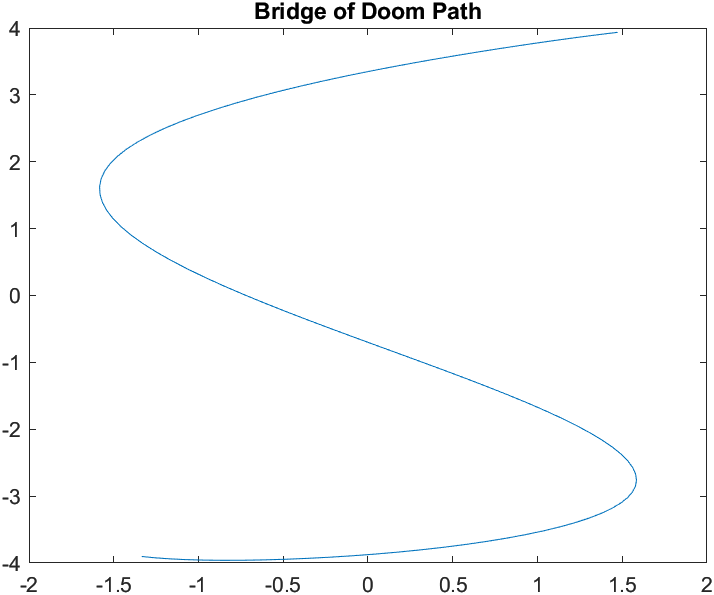
\includegraphics[width=0.65\textwidth]{img/predicted_path.png}
    \caption{The theoretical path that the Neato should have taken.}
    \label{fig:both_paths}
\end{figure}

\begin{figure}[h]
    \centering
    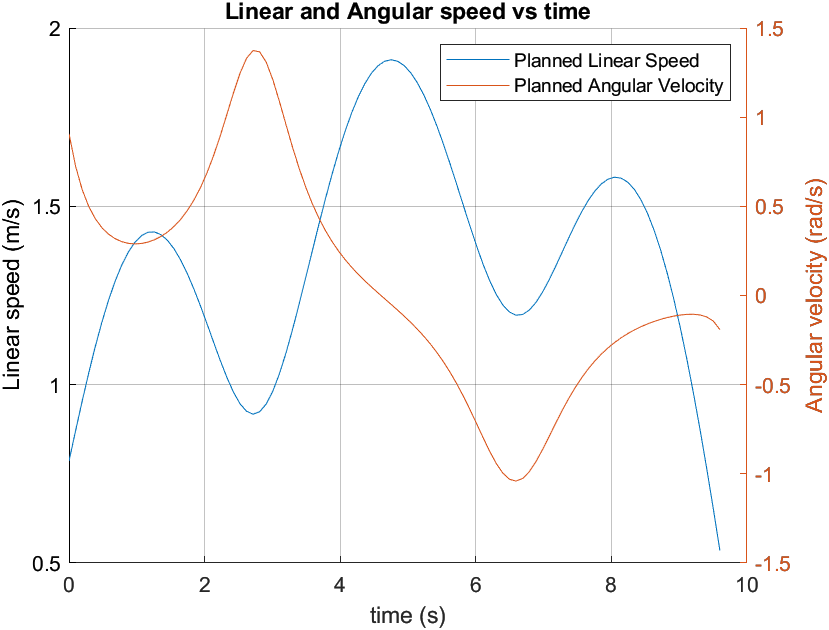
\includegraphics[width=0.65\textwidth]{img/planned_speeds.png}
    \caption{The theoretical linear speed and angular velocity about the z-axis (blue line and red line, respectively).}
    \label{fig:planned_lin_ang_speeds}
\end{figure}

\begin{figure}[h]
    \centering
    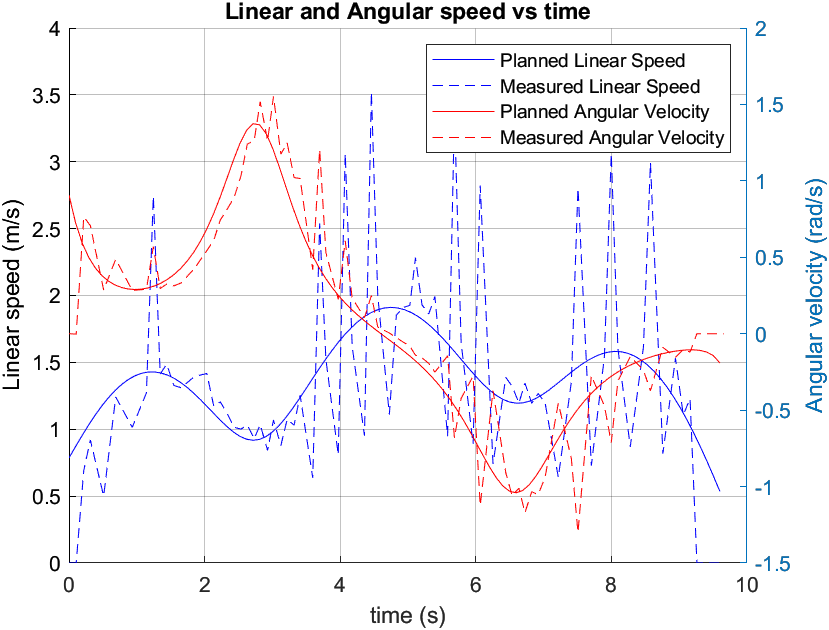
\includegraphics[width=0.65\textwidth]{img/measured_speeds.png}
    \caption{The theoretical linear speed and angular velocity about the z-axis (solid blue line and solid red line, respectively), plotted alongside the experimental linear speed and angular velocity (dashed blue line and dashed red line, respectively).}
    \label{fig:planned_wheelspeed1}
\end{figure}

\begin{figure}[h]
    \centering
    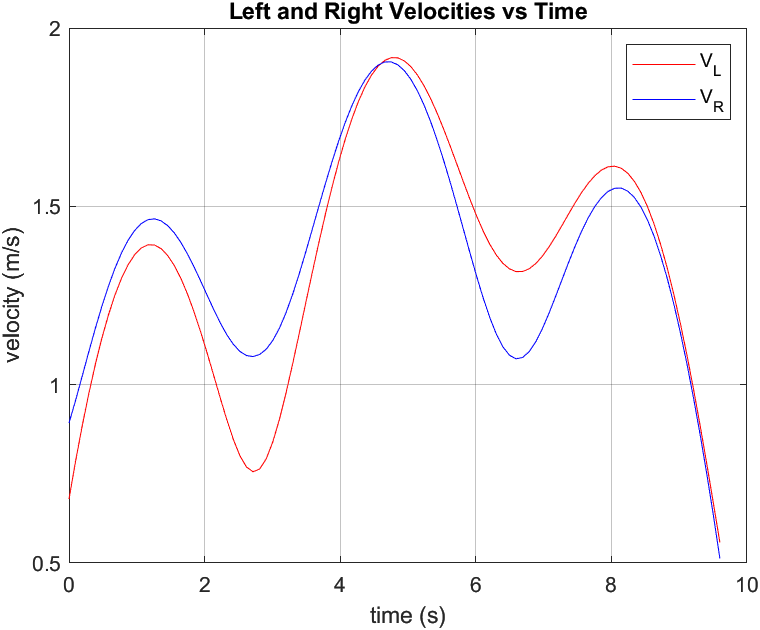
\includegraphics[width=0.65\textwidth]{img/planned_wheelspeed.png}
    \caption{The theoretical velocities of the left and right wheels (red line and blue line, respectively).}
    \label{fig:planned_wheelspeed2}
\end{figure}

\begin{figure}[h]
    \centering
    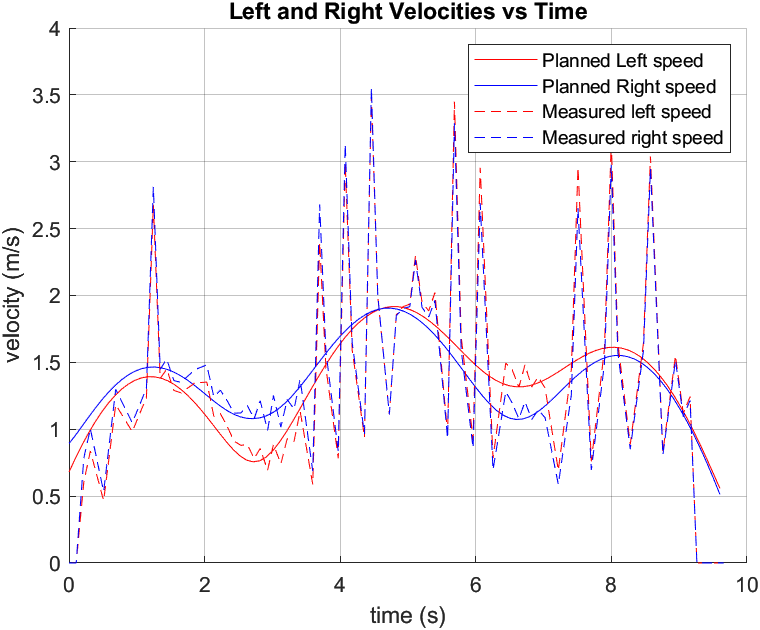
\includegraphics[width=0.65\textwidth]{img/measured_wheelspeeds.png}
    \caption{The theoretical velocities of the left and right wheels (solid red line and solid blue line, respectively), plotted alongside the experimental velocities of the left and right wheels (dashed red line and dashed blue line, respectively).}
    \label{fig:planned_wheelspeed3}
\end{figure}

\begin{figure}[h]
    \centering
    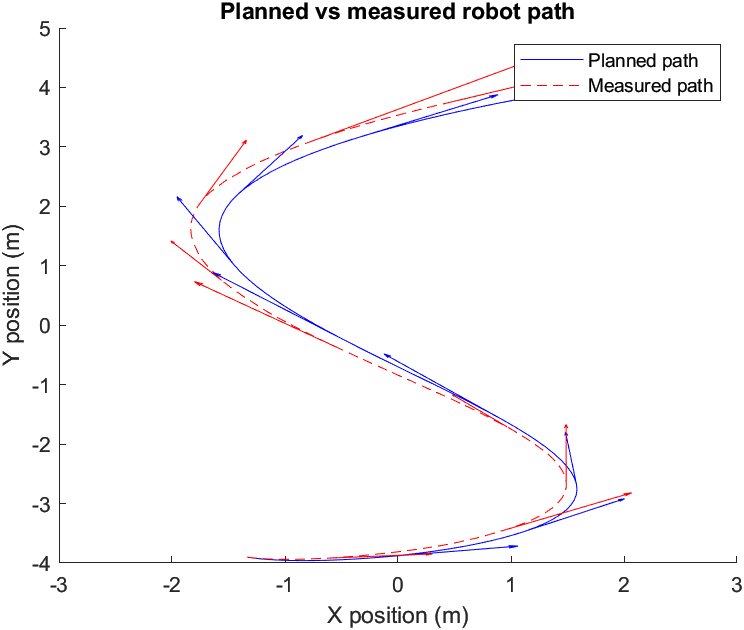
\includegraphics[width=0.65\textwidth]{img/measured_path.png}
    \caption{The predicted path (blue) and the measured path (dashed red). Also included are the velocity vectors at a few points on the curve.}
    \label{fig:planned_wheelspeed4}
\end{figure}



\end{document}